\subsection{アプリケーションの開発環境}
 webアプリケーション開発にはjavascriptのwebフレームワークである
Node.jsを用いた.Node.jsのパッケージであるExpressとnanoを用いた.
Expressはwebフレームワークで、nanoはCouchDBのためのドライバである.
その他に開発で使用したソフトを含めたバージョンなどの情報は付録に記載する.


\subsection{データベースの設計}
	CouchDBにss-mixの仕様書に記載されている
	データ格納方法およびデータ定義\cite{bibi1}に基づいてデータを格納する.
	CouchDBはひとつのデータベースの中に複数のドキュメントとよばれる
	データ構造を保持している.
	このドキュメントは事前にテーブルなどで定義する必要がなく,
	JSON形式であれば自由に記述できる.

	本研究ではひとつの医療行為に対してひとつのドキュメントで管理する.
	本研究で使用するドキュメントが保持する情報を表\ref{tab:doc}に示す.


	\begin{table}[htb]
		\begin{center}
			\caption{ドキュメントが保持する情報}
			\begin{tabular}{|l|c|r|r|}\hline
			Key & Value \\ \hline \hline
			id &  患者名、日付をドキュメントIDとしている. \\ \hline
			rev & \shortstack{ドキュメントの更新回数を示す. \\ 更新時に参照し競合を防ぐ.} \\ \hline
			name & 患者の名前 \\ \hline
			data & \shortstack{医療行為によって得られた情報を \\ json形式で格納.} \\ \hline
			\end{tabular}
			\label{tab:doc}
		\end{center}
	\end{table}


\subsection{アプリケーションの仕様}

	\subsubsection{新規のフォーマットのファイルに対するコスト}
	縦向き、横向きのcsv(地域の病院で生まれるような電子化された医療情報)
	の入力に対応している.
	行と列のどちらかに日付,他方に項目があると想定して入力ファイルから
	医療情報をキーと値に関連付けてデータベースに登録していく.

	電子カルテ固有の出力ファイルはHL7に対応していれば入力ファイルから
	医療情報をキーと値に関連付けてデータベースに登録していく.
	HL7の出力ファイルはパイプ区切りで,データの並び順に意味を持たせている.
	この並び順と項目,データを関連付けてキーと値に置き直して
	データベースに登録していく.

	このとき,HL7のデータの並び順と項目に関する情報が
	アプリケーション側で必要となる.
	つまり,異なる規格の医療情報を登録する際,
	そのフォーマットでデータをどのように意味付けしているかという情報を
	登録するコストが新規のフォーマットのファイルを
	アプリケーションに対応させるためにかかる.


	\subsubsection{同義キーの登録に対するコスト}
	医療情報の出力にはキーを関連付けるためのコストがかかる.
	これは新しいフォーマットで医療情報が入力されるたびに生まれる作業となる.
	これを医療関係者にさせることを想定している.
	(実装まだです.)


 %医療情報を収集するNoSQLデータベースシステム.UIとしてWebアプリを用意し,
	%医療関係者,薬剤師,患者の3者に対して,情報を扱いやすいようにした.

\subsection{患者情報閲覧}
	ユーザはログイン後,Accountタブから検索ワードを送信すると,
	/getdbでキーに検索ワードを値に含むキーと値の組を表示する.

	ここで,同義キーで管理されている項目群を表示するために
	キー同士の関連が登録されているドキュメントを参照している.
	\\
	\\



		\begin{figure}[htbp]
				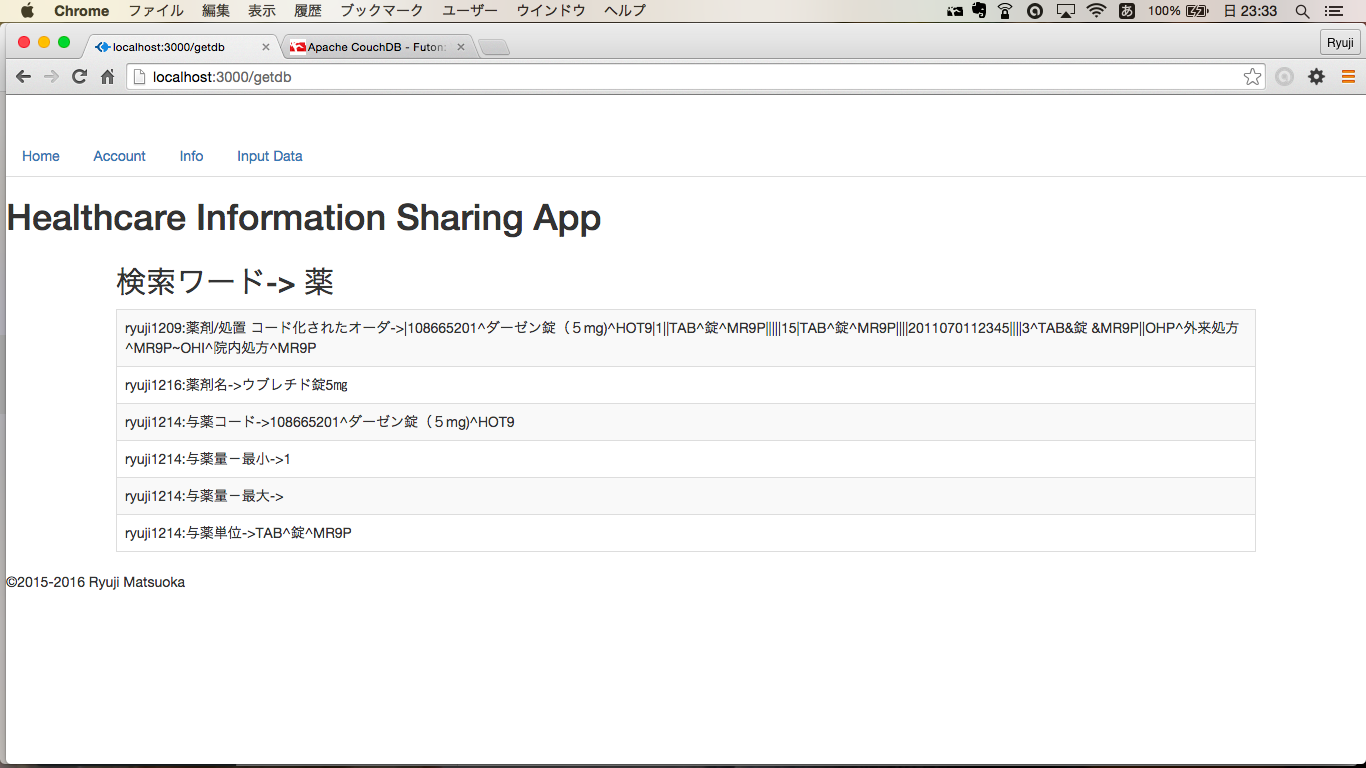
\includegraphics[width=5cm, bb=0 0 437 688]{./gazou/getdb.png}
			\caption{薬 でデータ抽出した様子}
			\label{ss-mix_sampledata}
		\end{figure}



\subsection{データの投入方法}
	ユーザはログイン後,Input Dataタブを選択する.
	次に入力するファイルを選択し,送信する\ref{fileiopage}.

	\begin{figure}[htbp]
		%\begin{center}
			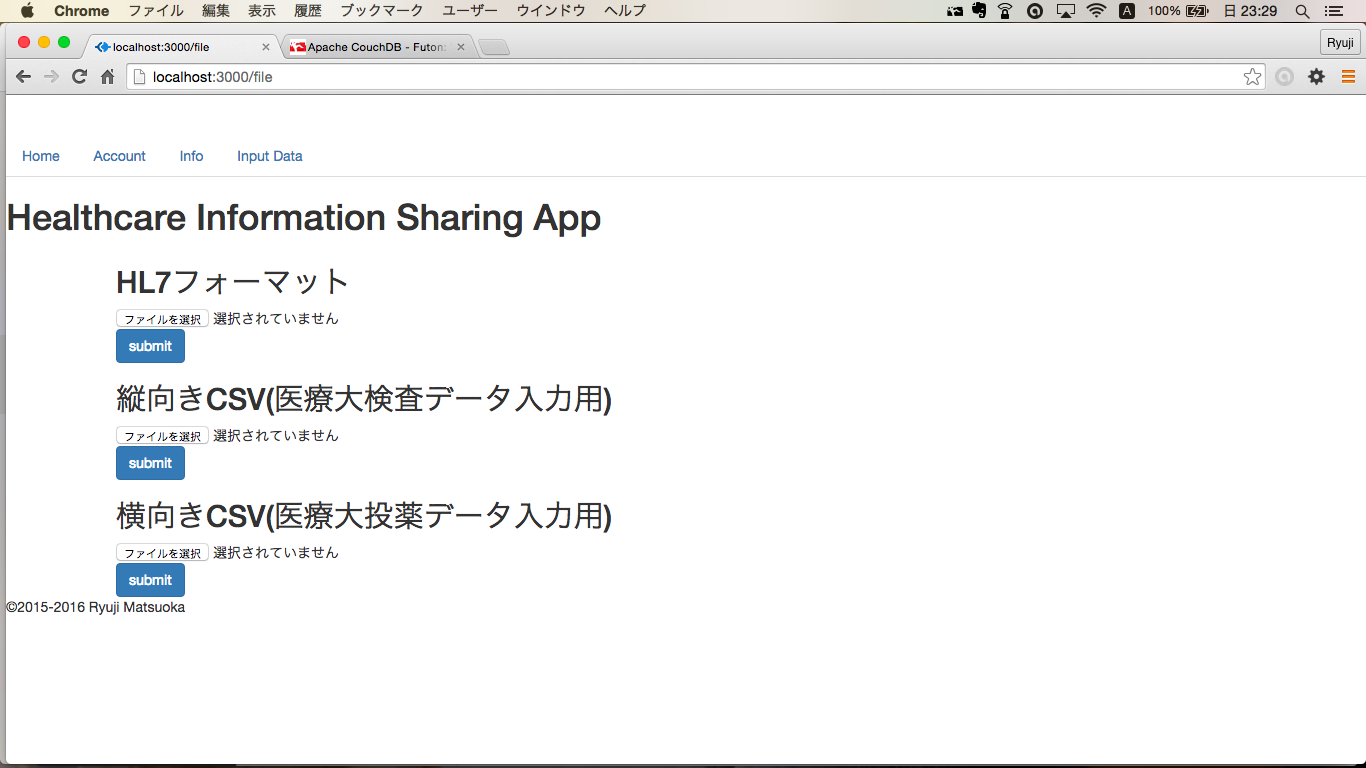
\includegraphics[width=5cm, bb=0 0 437 688]{./gazou/fileiopage.png}
		%\end{center}
		\caption{ファイル入力ページ}
		\label{fileiopage}
	\end{figure}

	1度の診療で1つのドキュメントを生成する.
	CSV入力ファイルに複数回の診療の記録があることを許容する.

		%\subsubsection{縦向きcsvファイルの場合}
		\subsubsection{CSVファイルの場合}
			CSVファイルは入力ファイルの行,列のどちらかに医療情報,
			他方に日付をとっているものを想定している.
			図\ref{csv-data-trans}は入力内容とCouchDBへの登録内容の
			対応を表したものである.

			\begin{figure}[htbp]
				%\begin{center}
					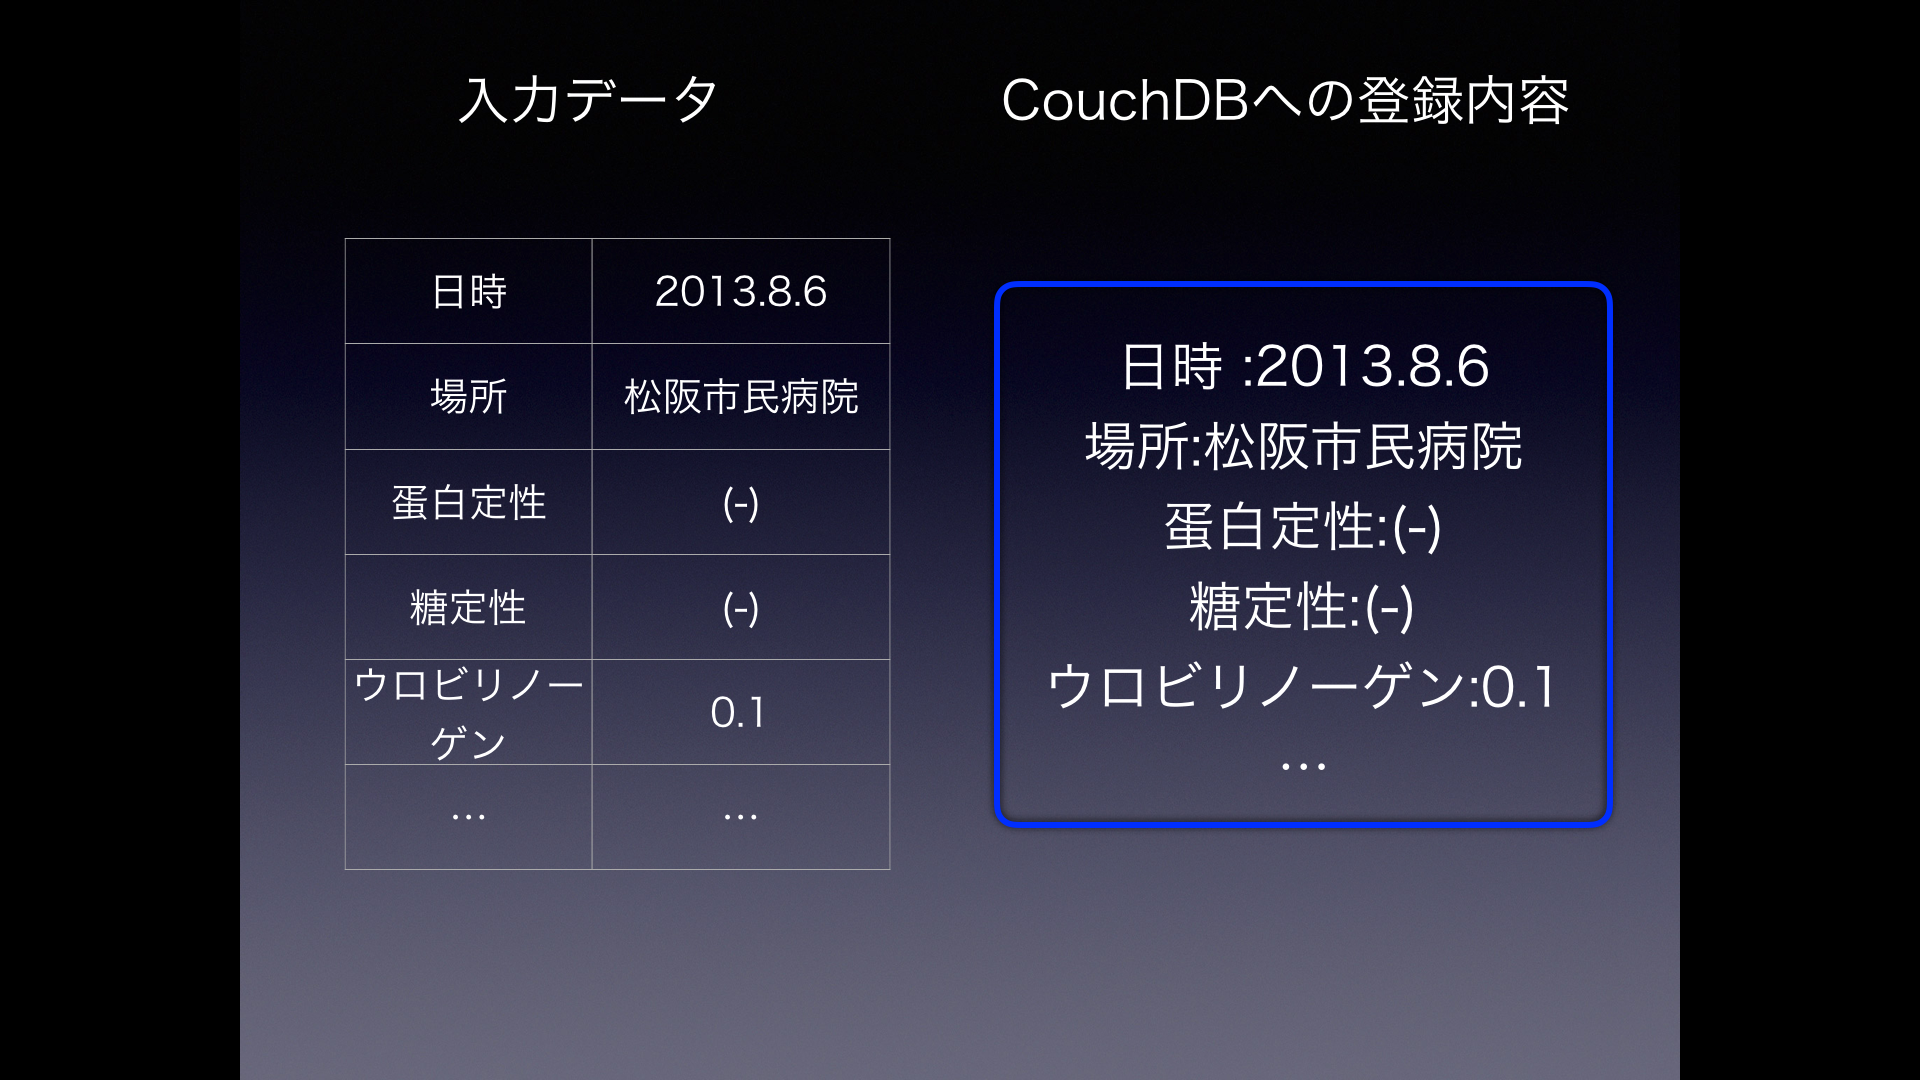
\includegraphics[width=5cm, bb=0 0 437 688]{./gazou/csv-data-trans.png}
				%\end{center}
				\caption{入力内容とDB登録内容の対応}
				\label{csv-data-trans}
			\end{figure}

			\begin{figure}[htbp]
				%\begin{center}
					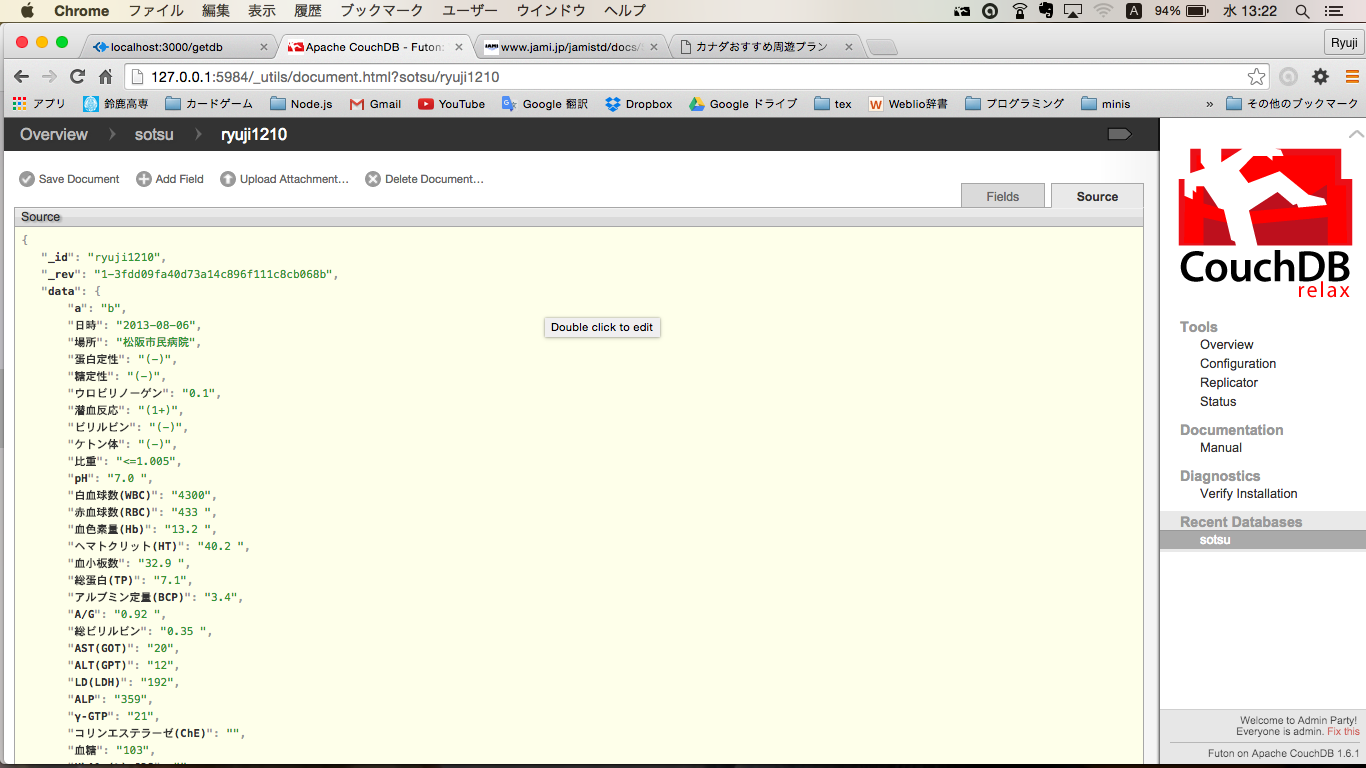
\includegraphics[width=5cm, bb=0 0 437 688]{./gazou/kensa.png}
				%\end{center}
				\caption{医療大の検査データ}
				\label{iryoudai-kensa-data}
			\end{figure}

		\if0
		\subsubsection{横向きcsvファイルの場合}
			holizontialparse
			医療大の投薬データ
		\fi


			\begin{figure}[htbp]
				%\begin{center}
					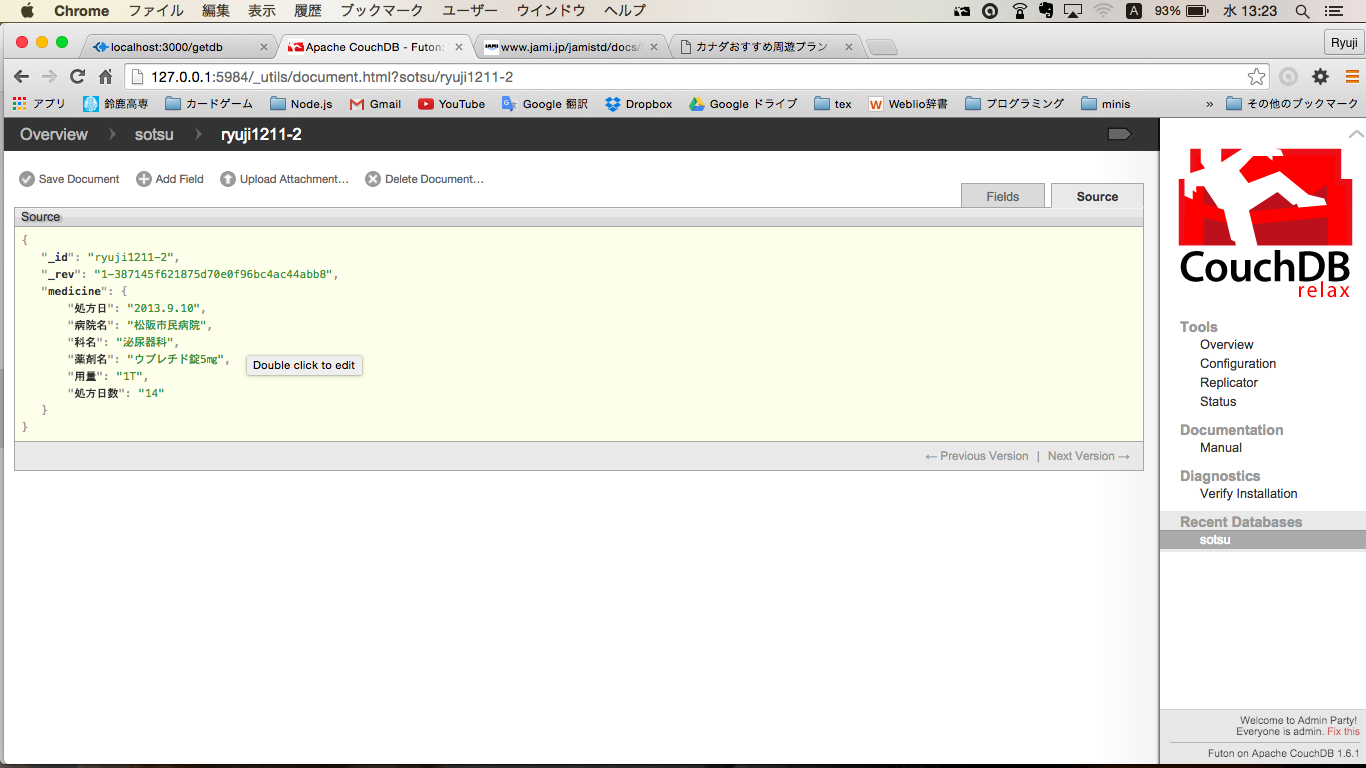
\includegraphics[width=5cm, bb=0 0 437 688]{./gazou/touyaku.png}
				%\end{center}
				\caption{医療大の投薬データ}
				\label{iryoudai-touyaku-data}
			\end{figure}

		\subsubsection{HL7ファイルの場合}
			前述のHL7のデータ定義に基づいて入力ファイルからデータを格納していく.

			HL7の出力ファイルはパイプ区切りで記述されており,
			並び順にデータの意味が割り振られている.
			図\ref{hl7-data-trans}の枠内のデータがOBX-3という
			セグメントのデータである.
			このセグメントの意味をアプリケーション内のテーブルから参照し,
			意味とデータをJSON形式に整形してCouchDBに登録する.



			本研究では医療規格にのっとっていない医療情報との関連付けを課題としている.
			そこでHL7にのっとったファイルからデータを抜き出し,
			データの配置によって割り振られている意味をキーとしてデータベースに
			格納していく.

			\begin{figure}[htbp]
				%\begin{center}
					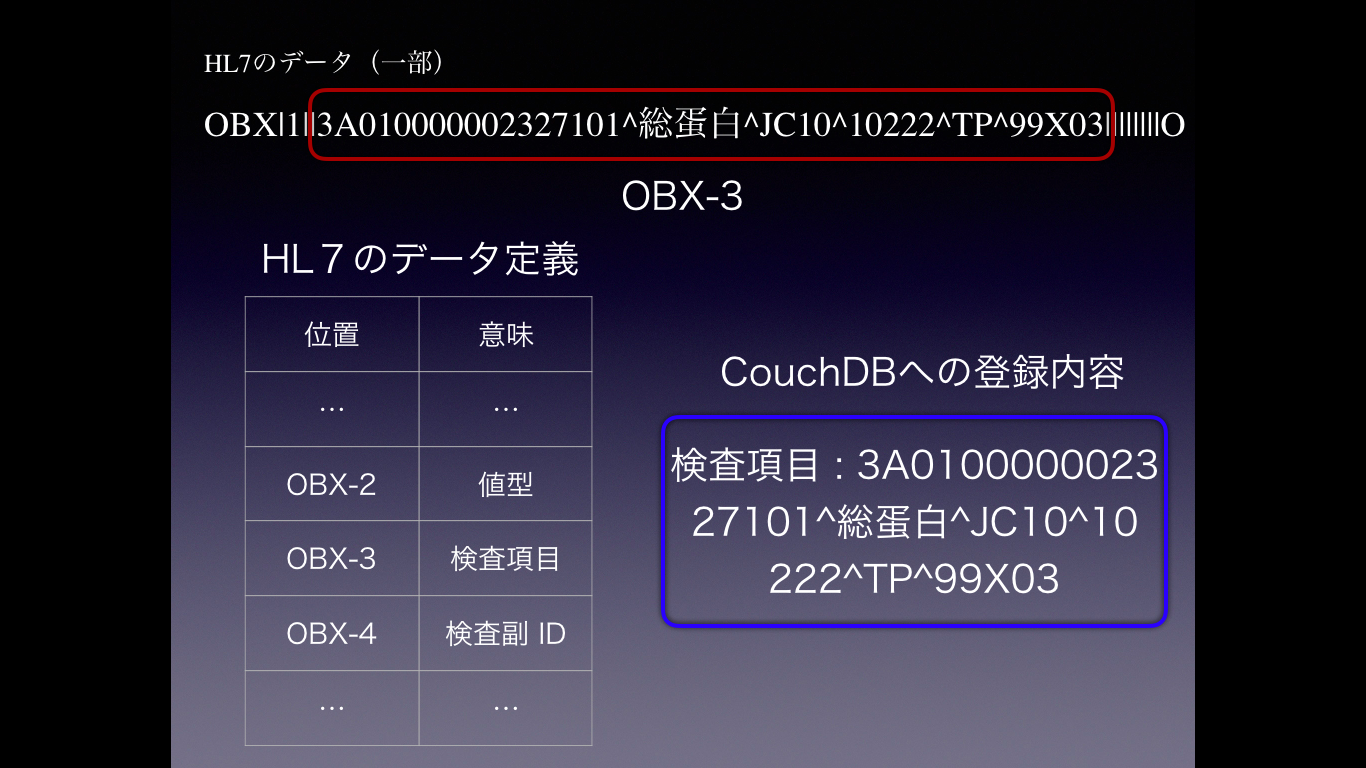
\includegraphics[width=5cm, bb=0 0 437 688]{./gazou/hl7-data-trans.png}
				%\end{center}
				\caption{HL7の生データからJSONへの変化}
				\label{hl7-data-trans}
			\end{figure}

			\begin{figure}[htbp]
				%\begin{center}
					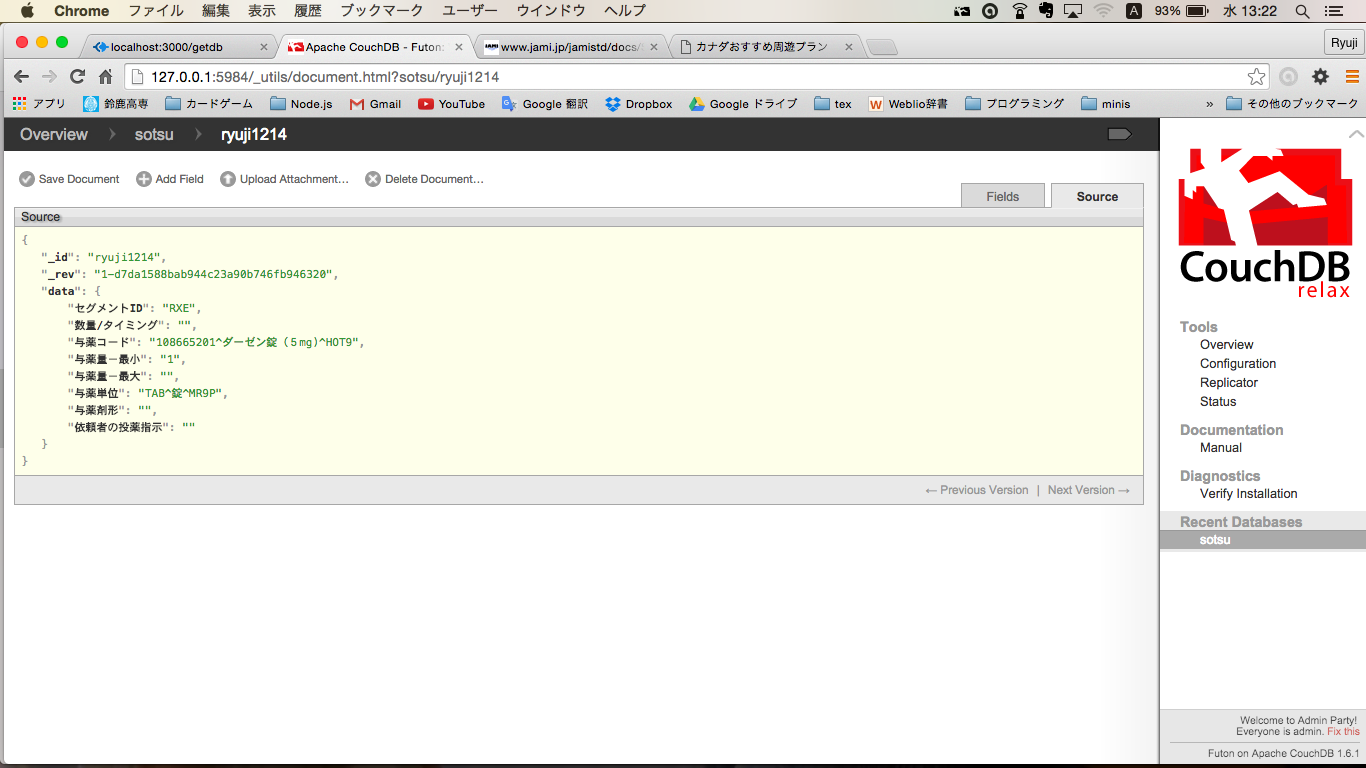
\includegraphics[width=5cm, bb=0 0 437 688]{./gazou/hl7.png}
				%\end{center}
				\caption{HL7のサンプルデータ}
				\label{hl7-data}
			\end{figure}



\subsection{同義キーの登録}
	データを参照するときに,キーが必要となる.キーには様々な意味を持つものがあるが,
	異なる規格のデータでは同じ情報を指し示すキーであっても,
	異なるキーが使われている.
	これは新規の規格が医療情報ソフトに流入するたびに課題となる.

	そこで,本研究ではユーザによる同義キーの登録の機能を用意した.
	ユーザは同義である2つのキーを入力すると
	それが同義キーを管理するドキュメントに追加される.

	図\ref{relation}では投薬データの処方日と診断データの日時が同義として登録されている.
	図\ref{relationApp}では検索ワードは処方であるので
	処方をキーに含むデータが検索結果として表示される.
	さらに,検索結果に処方日があり,これは日時と同義として登録されているため,
	日時のデータも検索結果として表示される.
	(実装まだですが.texが嫌になった時にやります。
	仕様としては、処方日、日時ともにその右に日付がならびます。)

	\begin{figure}[htbp]
			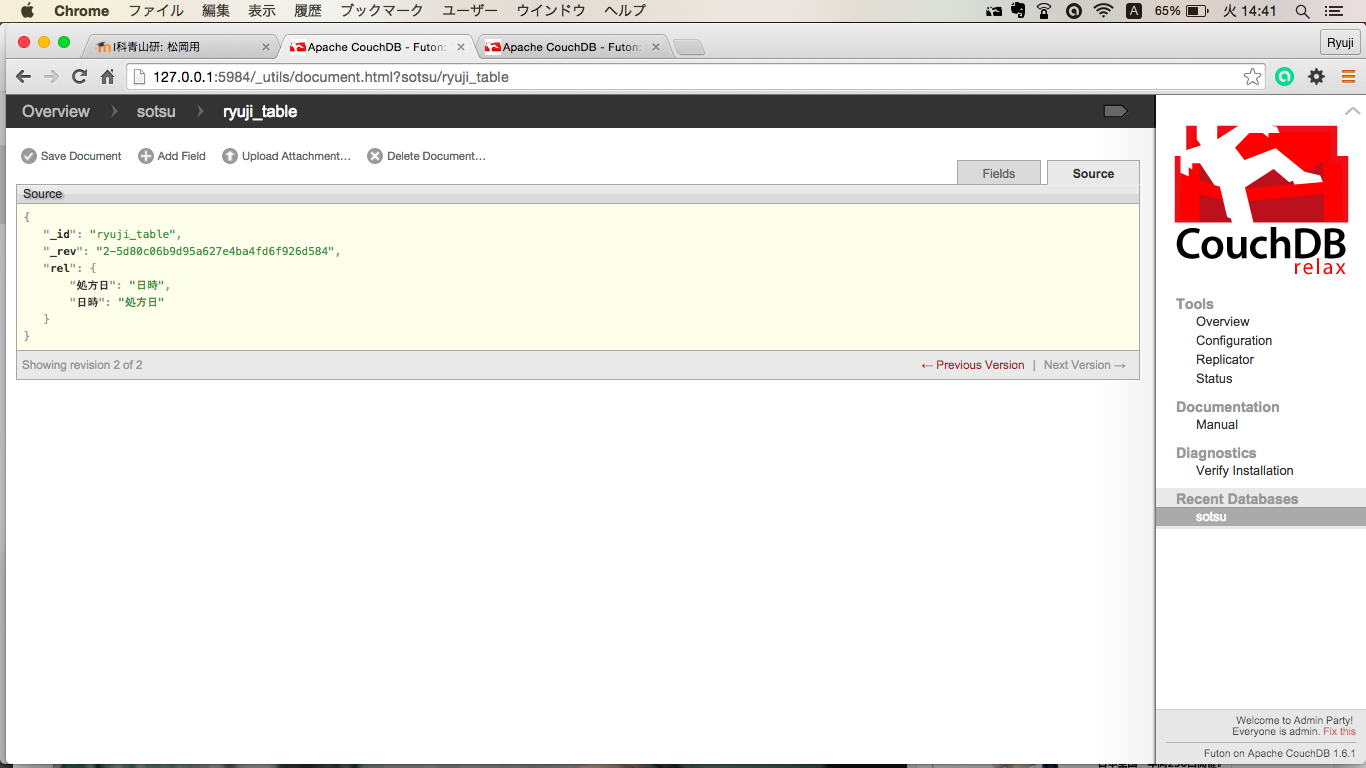
\includegraphics[width=5cm, bb=0 0 437 688]{./gazou/relation.png}
		\caption{同義キーを管理するドキュメント}
		\label{relation}
	\end{figure}

	\begin{figure}[htbp]
		%\begin{center}
			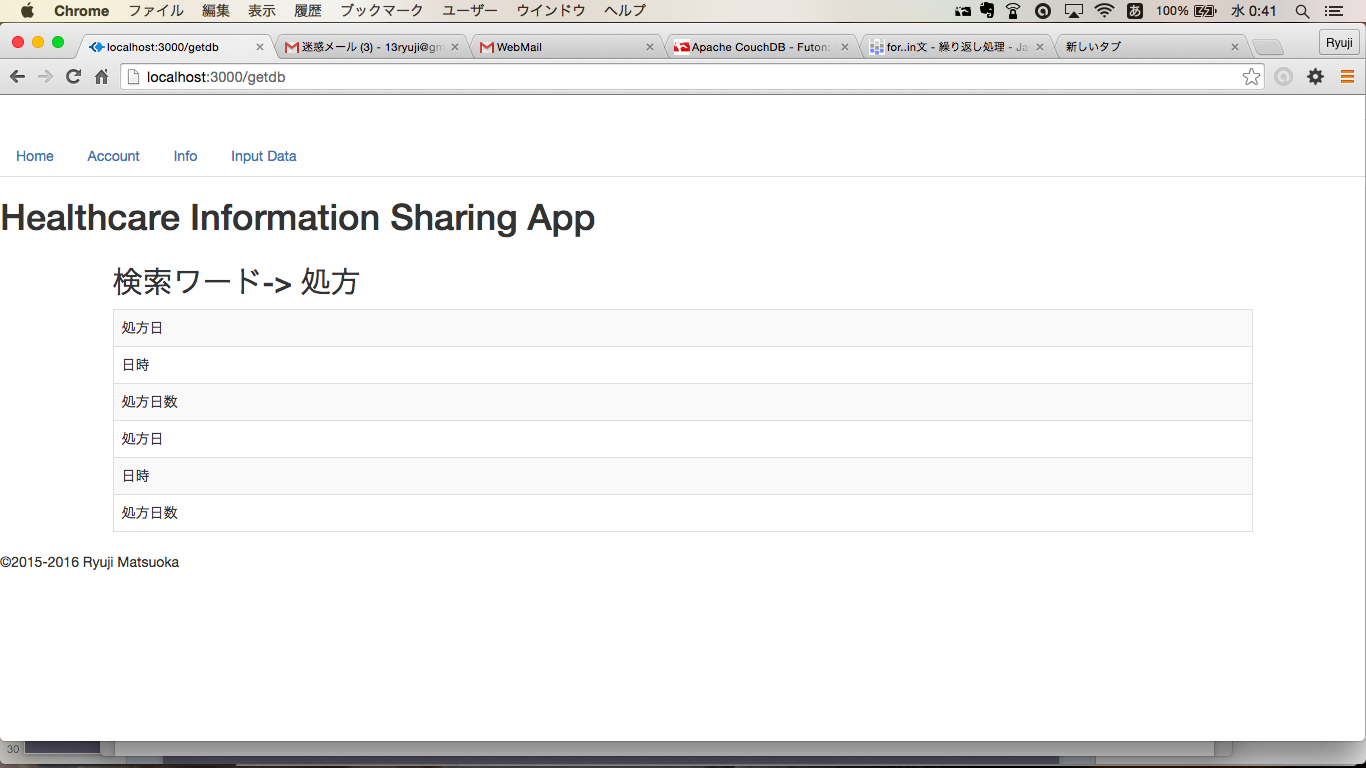
\includegraphics[width=5cm, bb=0 0 437 688]{./gazou/relationApp.png}
		%\end{center}
		\caption{処方と検索して同義キーとして登録されている日時を表示する}
		\label{relationApp}
	\end{figure}
